
\documentclass[twocolumn]{article}

\usepackage{graphicx} % Required for inserting images
\usepackage{amsmath}
\usepackage{amssymb}
\usepackage{url}
\usepackage[a4paper, left=1.5cm, right=1.5cm, top=2.5cm, bottom=2.5cm]{geometry}
\usepackage{etoolbox}
\usepackage{booktabs}

\patchcmd{\thebibliography}{\section*{\refname}}{}{}{}

\title{Naive Bayes classifier applied to paranormal stories}

\author{
Alan Fernando Bravo Pimentel \and
Gonzalo Makenly Higuera Inzunza \and
Juan Pablo de la Peña Gonzalez \and
Sarah Camila Guzmán Fierro \and
Miguel Angel Rivas Torres
}

\date{Semptember 14th 2025}

\begin{document}

\maketitle

\begin{abstract}
Online websites act as repertoires of reports of paranormal experiences, offering a distinctive set of information on cultural beliefs and individual perceptions. This study aims to  explore the use of Natural Language Processing (NLP) techniques to categorize such stories. A Naive Bayes classifier was trained to predict the type of phenomena described. The data acquisition process involved web scraping and drew information from the \textit{Your Ghost Stories} platform, the text was then processed using a count vectorizer. Several iterations of the naive Bayes classifier were tested, and several accuracy metrics were utilized for evaluating the model's performance.  

The findings suggest that while the two first classifiers using the packages \textit{naivebayes} and \textit{e1071} obtained rather poor results, the other more sophisticated models that included a simplification of the categories as well as further tweaks such as making use of Laplace Smoothing obtained better results overall. More precisely, it was noticed that even in the best model, metrics like F1, recall and precision were not excellent, despite the accuracy being 0.7202. This showcases potential limitations of the approach in use and at the same time highlights the potential applicability of these tools to NLP analysis.


\end{abstract}

\section{Introduction}
Throughout human history, paranormal narratives have captured the imagination of individuals all over the world. Stories of supernatural phenomena, haunted places, and spiritual encounters have been commonplace elements of folklore and constitute a form of cultural data. For this reason, several websites and platforms have emerged with the mission of storing and showcasing this wide variety in the digital era. Among these, the platform \textit{Your Ghost Stories} offers thousands of individual accounts of paranormal experiences submitted by users. Undeniably, these stories provide a highly interesting and rich framework for applying computational tools to explore, analyze, and structure information in the form of text.
The primary goal of this study is to train and implement a naive Bayes classifier capable of categorizing paranormal stories according to the type of phenomenon described. In order to accomplish this, we built a dataset by performing web scraping on the website \textit{Your Ghost Stories}. Afterward, some techniques of natural language processing were employed, such as tokenization, and a sparse matrix prepared the data for further analysis. 
A naive Bayes classifier was then appiled to this dataset, taking advantage of its effectiveness for text classification applications. By modeling the distribution of words from different categories of these stories, the classifier can predict the type of event described in each story. The performance of this classifier was later evaluated through several metrics. \\
This study demonstrates the capabilities of NLP techniques coupled with probabilistic modeling in text to explore the way that paranormal stories are shared and categorized.


\section{Methodology}
In order to acquire the data for the classifier, we employed web scraping to extract stories from the \textit{Your Ghost Stories} website. The first step was to verify scraping permission using the paths\_allowed() function from the robotstxt package in R. Then, the script used managed to identify the relevant elements to capture such as the title of each story, its description as well as other relevant data such as country, state, and category. Additionally, a custom function called get\_story() was implemented so as to automate the process and extract multiple stories in parallel, which increased efficiency. The resulting dataset was composed in an organized table that contains fields for id, title, country, state, category and description. Lastly, the data were exported to a CSV file. \\
The preparation of the text for analysis began with each story being tokenized in turn, allowing the narrative descriptions to be broken down into discrete words. Then, the most common stop words were eliminated and Only the most instructive terms remained in the text. A frequency count of the words that appeared in each document was then produced, offering a systematic method of  expressing the narratives numerically. These word counts were then transformed into a sparse matrix, where each row corresponded to a story and each column represented a unique word (feature). The entries of the matrix indicated the frequency of each word inside a particular story. 
Finally, the categories associated with each story were aligned with the rows of the newly created sparse matrix, so that we could create a dataset in which we could represent the information quantitatively and keep it linked to its respective class label.
Afterward, a naive Bayes Classifier was trained on the dataset. This classifier relies the assumption of conditional independence between features, which in practice means that the presence of one word in a document is considered independent of the presence of any other word given the category. The classifier also relies on the Bayes Theorem to calculate the probability that a certain observation belongs to a class.
In particular, given a new observation, 
\( \tilde{\boldsymbol{x}} = (\tilde{x}_{1}, \dots, \tilde{x}_{p})^{\intercal}\tilde{\boldsymbol{x}}.\)
we compute
\[
\mathbb{P}(Y = k \mid \boldsymbol{X} = \tilde{\boldsymbol{x}}) = \frac{\mathbb{P}(Y = k)f(\tilde{\boldsymbol{x}} \mid y = k)}{\sum_{k = 1}^{K} \mathbb{P}(Y = k)f(\tilde{\boldsymbol{x}} \mid y = k)}
\]



The implementation was carried out using several approaches including the "naivebayes" package in R. As per usual, the training set was defined by randomly sampling 70\% of the data, while the other 30\% was reserved for testing. The performance of our classifier was then evaluated using accuracy, precision, recall, and F1-score to capture overall performance when predicting and performance in individual categories.
Finally, certain improvements were made to fix common problems with text classification.  The Poisson distribution was investigated so that it could be used as a substitute for the standard assumption in the naive Bayes model as word counts are discrete and sometimes sparse. Another tool employed was Laplace smoothing and it was also used to manage the zeros in the matrix and prevent zero classification probabilities. Cross-validation techniques were also used and helped us find the smoothing parameter's most optimal value and improve the performance of the classifier.



\section{Application}
During the web scrapping process, up to 20,125 different observations/stories were retrieved. As mentioned in the methodolgy, a sparse matrix was built using those data, this sparse matrix represented every word as a column and showed how frequently the words show up in each story. However, due to computational limits, this sparse matrix was reduced to only the 3000 most frequent words. In addition to that, all categories were joined together and appended to the sparse matrix before turning it into a dataframe. Note that null values were removed and some stories were discarded, leaving us with 20,106 usable stories. Figures 1-3 on the right show the most frequent combinations of 1, 2 and 3 words across all categories.
\begin{figure}[htbp]
    \centering
    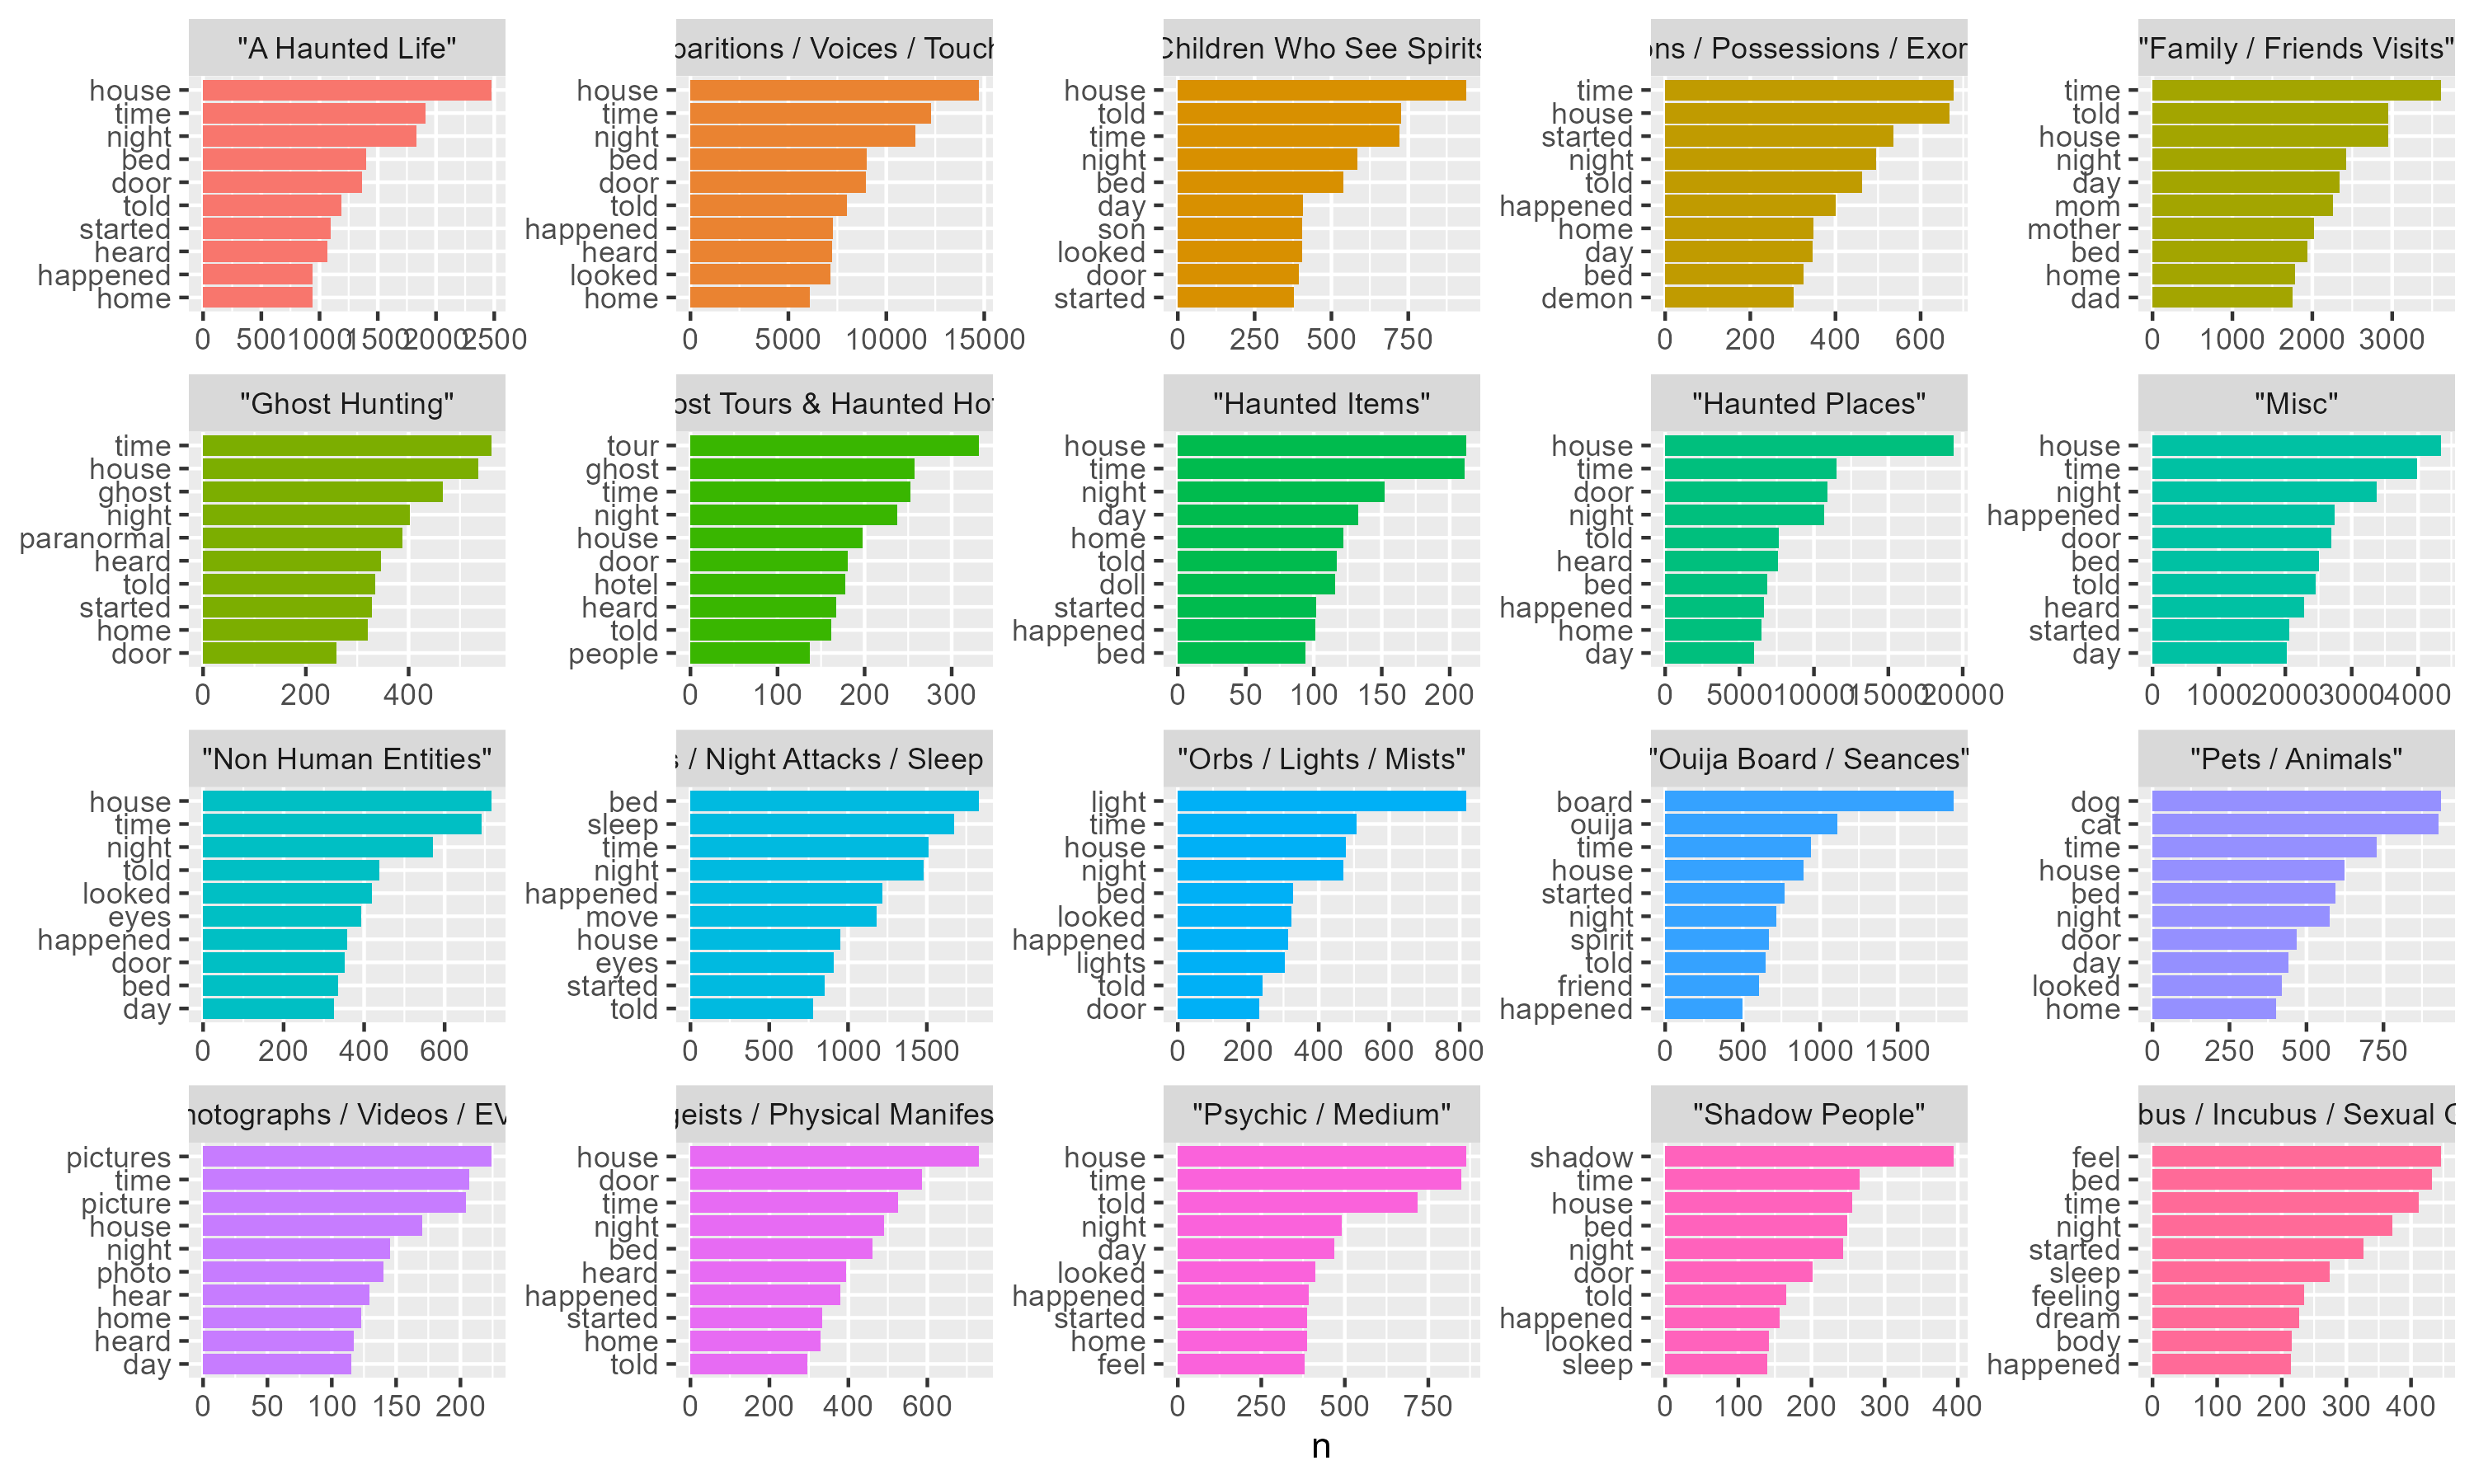
\includegraphics[width=1\columnwidth]{figures/unigrams.png}
    \caption{10 most frequent words}
    \label{unigrams}
\end{figure}

\begin{figure}[htbp]
    \centering
    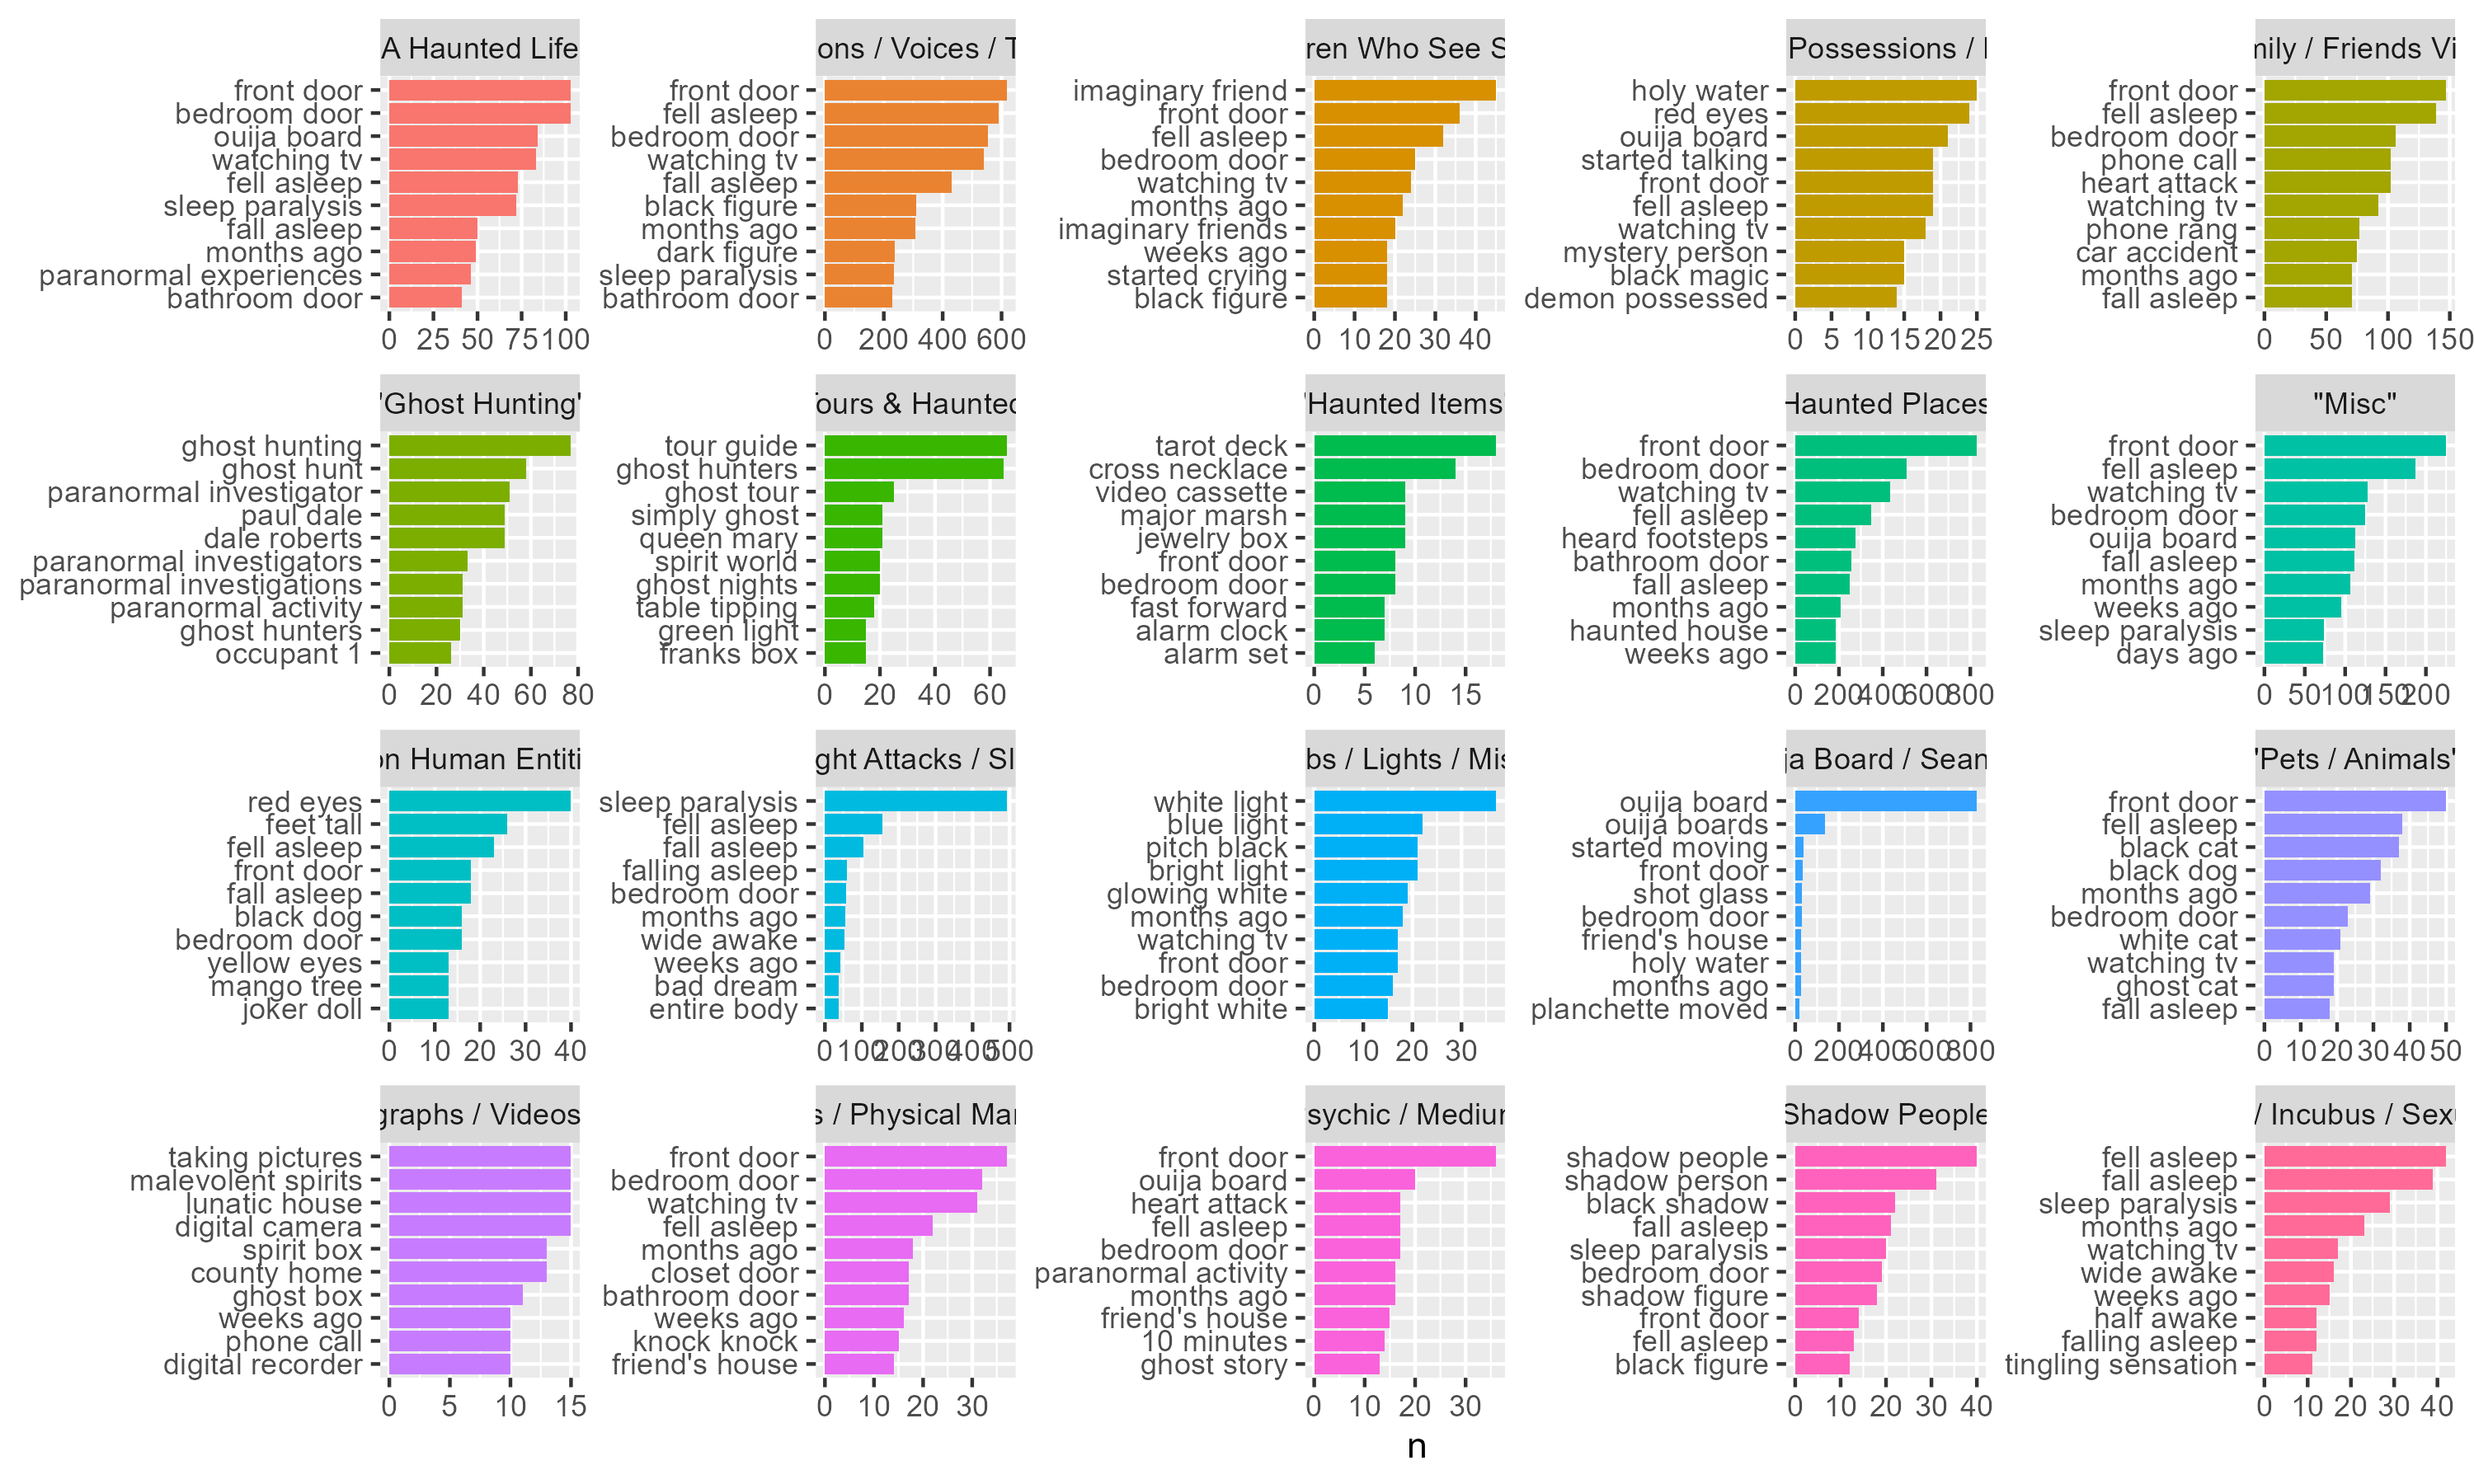
\includegraphics[width=1\columnwidth]{figures/bigrams.png}
    \caption{10 most frequent combinations of two words}
    \label{unigrams}
\end{figure}

\begin{figure}[htbp]
    \centering
    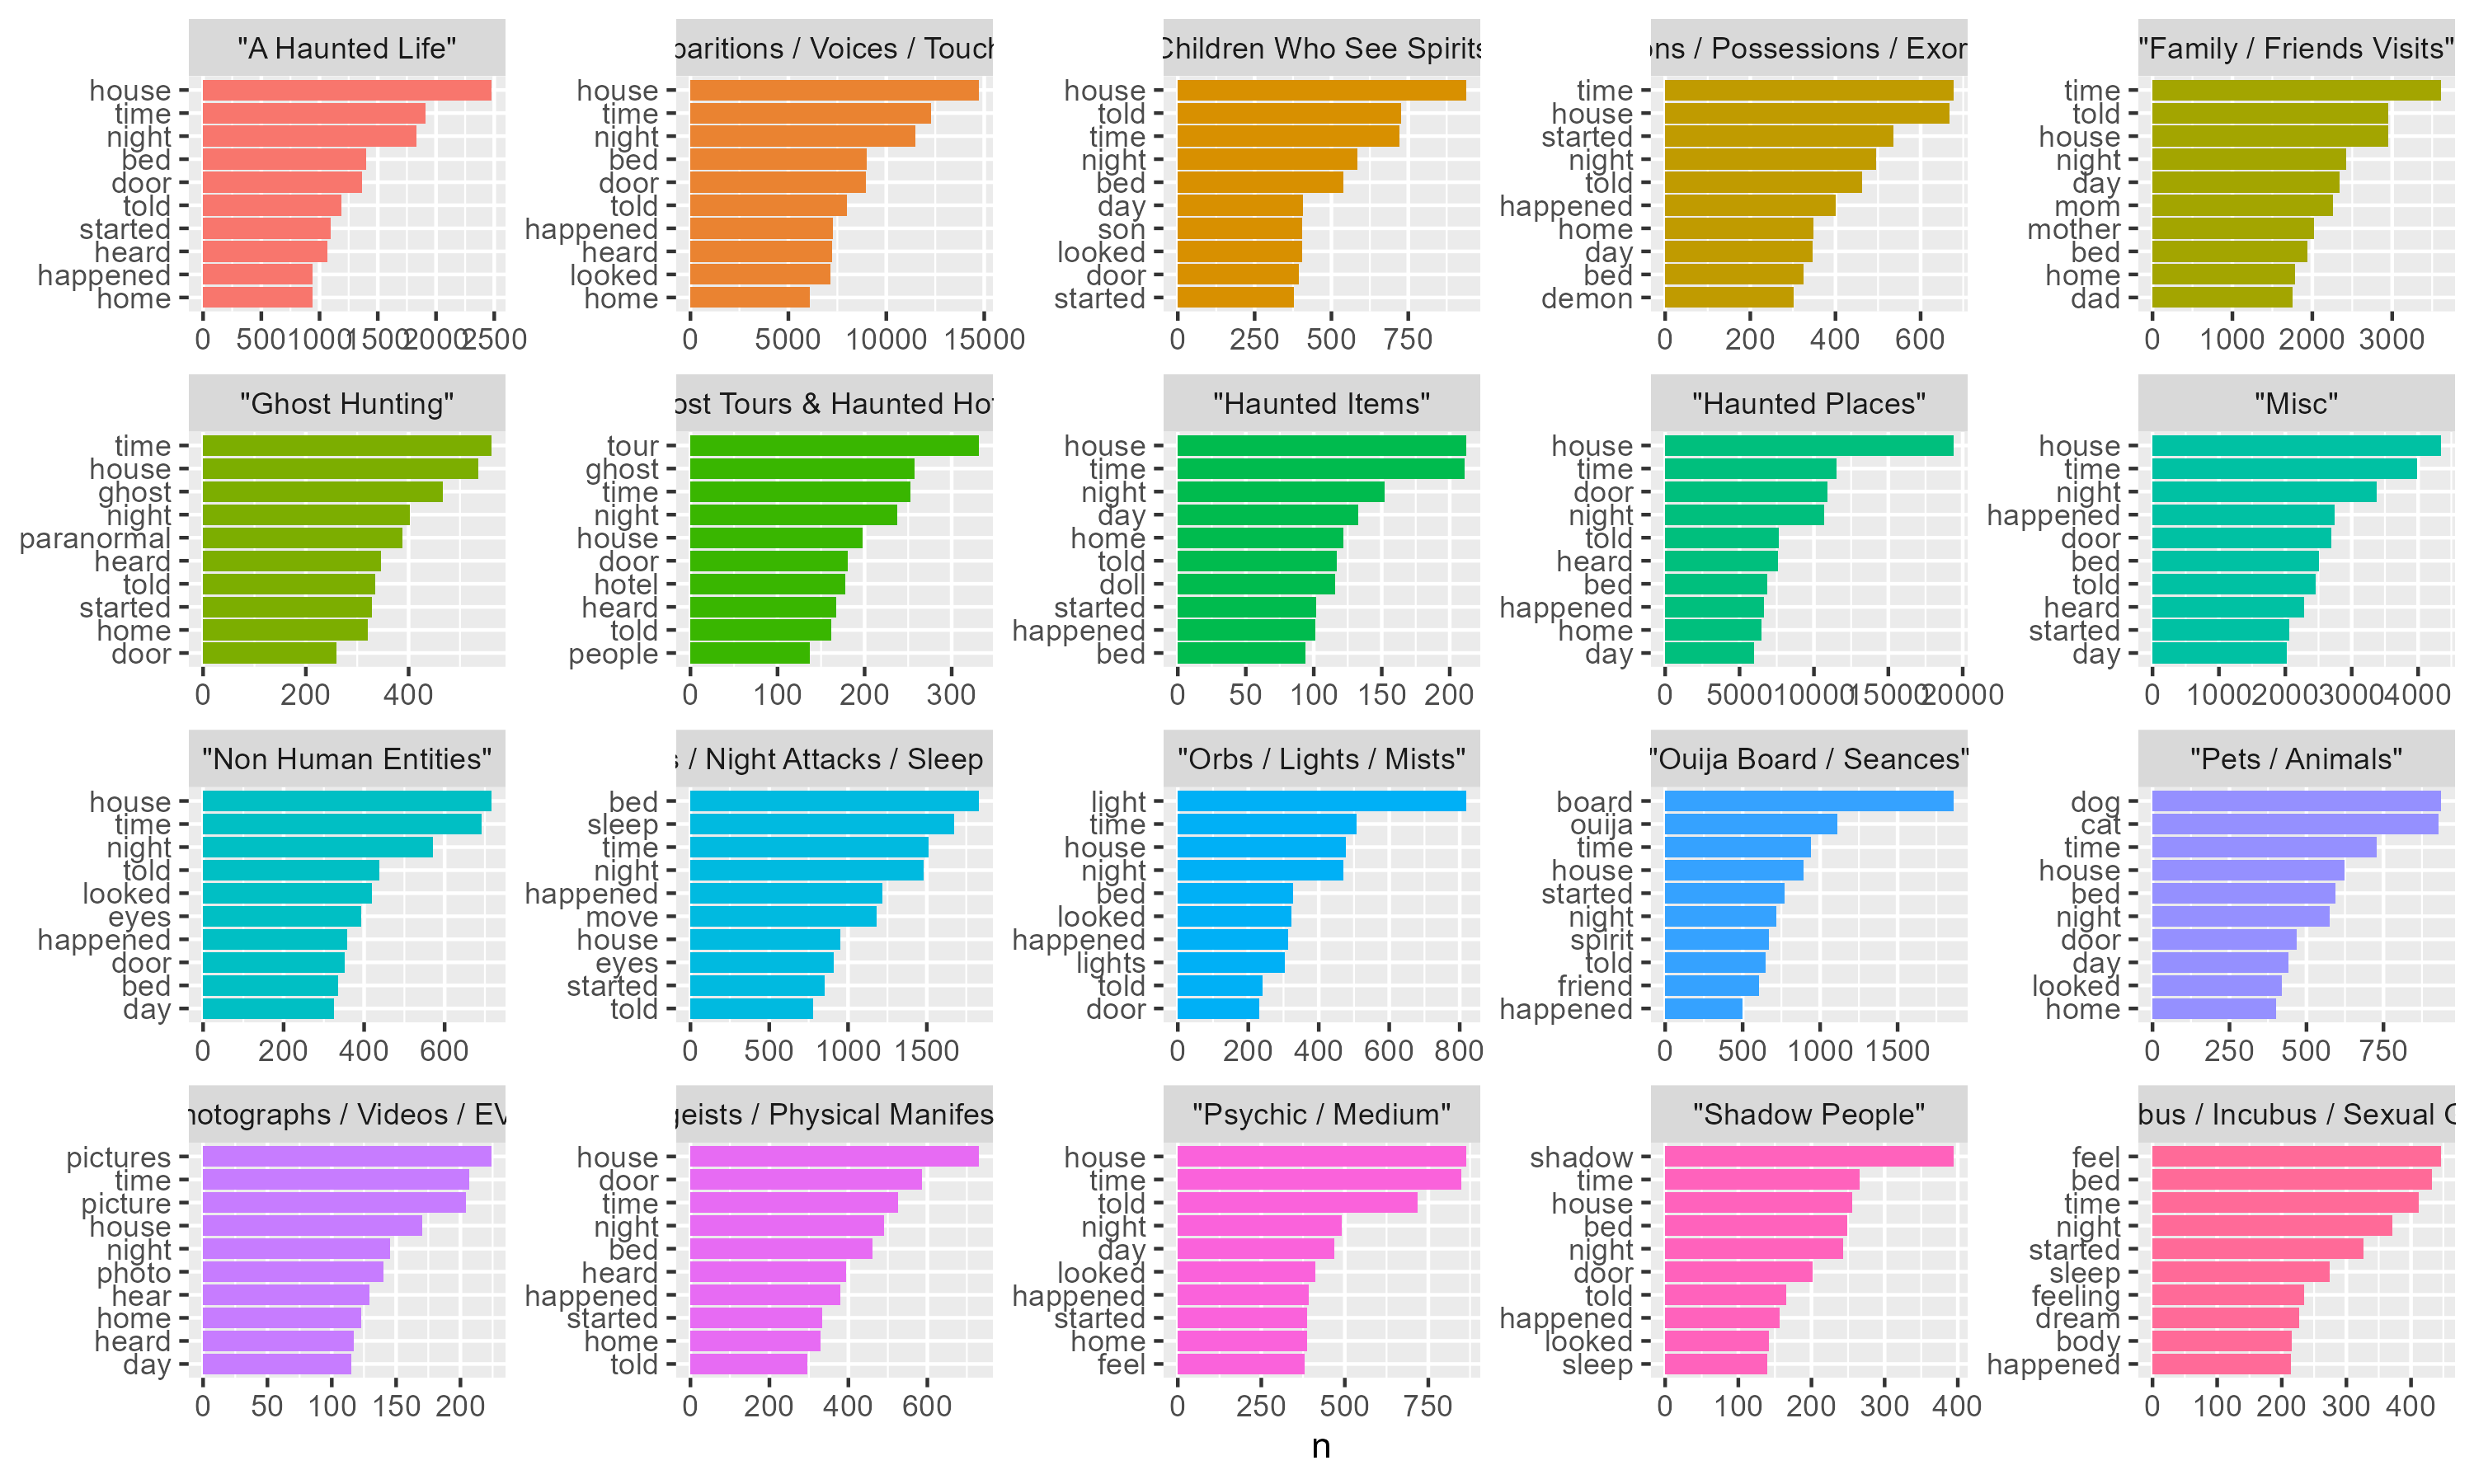
\includegraphics[width=0.9\columnwidth]{figures/unigrams.png}
    \caption{10 most frequent combinations of three words}
    \label{unigrams}
\end{figure}

With this organized information available, several iterations of a naive Bayes classifier were trained on this data. The first one of which being a model trained using the library e1071 which yielded the following results:
\begin{table}[h]
\centering
\caption{Overall e1071 classifier performance metrics.}
\small
\resizebox{\columnwidth}{!}{
\begin{tabular}{lccccccc}
\toprule
Accuracy & Macro Precision & Macro Recall & Macro F1 & Micro Precision & Micro Recall & Micro F1 \\
\midrule
0.0109 & 0.4996 & 0.0860 & 0.0575 & 0.0109 & 0.0109 & 0.0109 \\
\bottomrule
\end{tabular}
}
\end{table}
\begin{table}[h]
\centering
\caption{Per-class precision, recall, F1 score, and support of e1071 model.}
\small
\resizebox{\columnwidth}{!}{
\begin{tabular}{lcccc}
\toprule
Class & Precision & Recall & F1 & Support \\
\midrule
A Haunted Life & 1.0000 & 0.0057 & 0.0114 & 175 \\
Apparitions / Voices / Touches & NaN & 0.0000 & NA & 1926 \\
Children Who See Spirits & NaN & 0.0000 & NA & 119 \\
Demons / Possessions / Exorcisms & 0.5000 & 0.0112 & 0.0220 & 89 \\
Family / Friends Visits & NaN & 0.0000 & NA & 555 \\
Ghost Hunting & 1.0000 & 0.0156 & 0.0308 & 64 \\
Ghost Tours \& Haunted Hotels & 0.3846 & 0.1087 & 0.1695 & 46 \\
Haunted Items & 0.0077 & 0.5417 & 0.0151 & 24 \\
Haunted Places & NaN & 0.0000 & NA & 1440 \\
Misc & NaN & 0.0000 & NA & 648 \\
Non Human Entities & NaN & 0.0000 & NA & 86 \\
Old Hags / Night Attacks / Sleep Paralysis & NaN & 0.0000 & NA & 206 \\
Orbs / Lights / Mists & NaN & 0.0000 & NA & 83 \\
Ouija Board / Seances & NaN & 0.0000 & NA & 116 \\
Pets / Animals & NaN & 0.0000 & NA & 106 \\
Photographs / Videos / EVP & 0.0964 & 0.1667 & 0.1221 & 48 \\
Poltergeists / Physical Manifestations & NaN & 0.0000 & NA & 88 \\
Psychic / Medium & NaN & 0.0000 & NA & 118 \\
Shadow People & 0.0083 & 0.8333 & 0.0164 & 42 \\
Succubus / Incubus / Sexual Ghosts & 1.0000 & 0.0377 & 0.0727 & 53 \\
\bottomrule
\end{tabular}
}
\end{table}


On the other hand, the results obtained by the classifier that used the "naivebayes" package in R were the following:
\begin{table}[h]
\centering
\caption{Overall classifier performance metrics of naivebayes model.}
\small
\resizebox{\columnwidth}{!}{
\begin{tabular}{lccccccc}
\toprule
Accuracy & Macro Precision & Macro Recall & Macro F1 & Micro Precision & Micro Recall & Micro F1 \\
\midrule
0.0109 & 0.4996 & 0.0860 & 0.0575 & 0.0109 & 0.0109 & 0.0109 \\
\bottomrule
\end{tabular}
}
\end{table}
\begin{table}[h]
\centering
\caption{Per-class precision, recall, F1 score, and support of naivebayes model.}
\small
\resizebox{\columnwidth}{!}{
\begin{tabular}{lcccc}
\toprule
Class & Precision & Recall & F1 & Support \\
\midrule
A Haunted Life & 1.0000 & 0.0057 & 0.0114 & 175 \\
Apparitions / Voices / Touches & NaN & 0.0000 & NA & 1926 \\
Children Who See Spirits & NaN & 0.0000 & NA & 119 \\
Demons / Possessions / Exorcisms & 0.5000 & 0.0112 & 0.0220 & 89 \\
Family / Friends Visits & NaN & 0.0000 & NA & 555 \\
Ghost Hunting & 1.0000 & 0.0156 & 0.0308 & 64 \\
Ghost Tours \& Haunted Hotels & 0.3846 & 0.1087 & 0.1695 & 46 \\
Haunted Items & 0.0077 & 0.5417 & 0.0151 & 24 \\
Haunted Places & NaN & 0.0000 & NA & 1440 \\
Misc & NaN & 0.0000 & NA & 648 \\
Non Human Entities & NaN & 0.0000 & NA & 86 \\
Old Hags / Night Attacks / Sleep Paralysis & NaN & 0.0000 & NA & 206 \\
Orbs / Lights / Mists & NaN & 0.0000 & NA & 83 \\
Ouija Board / Seances & NaN & 0.0000 & NA & 116 \\
Pets / Animals & NaN & 0.0000 & NA & 106 \\
Photographs / Videos / EVP & 0.0964 & 0.1667 & 0.1221 & 48 \\
Poltergeists / Physical Manifestations & NaN & 0.0000 & NA & 88 \\
Psychic / Medium & NaN & 0.0000 & NA & 118 \\
Shadow People & 0.0083 & 0.8333 & 0.0164 & 42 \\
Succubus / Incubus / Sexual Ghosts & 1.0000 & 0.0377 & 0.0727 & 53 \\
\bottomrule
\end{tabular}
}
\end{table}


As we can see,there were no noticeable differences.


After incorporating the case\_when() function and in doing so simplifying the categories, the results for both models were:
\vspace{5cm}
\begin{table}[h]
\centering
\caption{Overall classifier performance metrics (simplified categories) e1071.}
\small
\resizebox{\columnwidth}{!}{
\begin{tabular}{lcccccc}
\toprule
Accuracy & Macro Precision & Macro Recall & Macro F1 & Micro Precision & Micro Recall & Micro F1 \\
\midrule
0.7202 & 0.4452 & 0.4914 & 0.4672 & 0.7202 & 0.7202 & 0.7202 \\
\bottomrule
\end{tabular}
}
\end{table}
\begin{table}[h]
\centering
\caption{Per-class precision, recall, F1 score, and support (simplified categories) e1071.}
\small
\resizebox{\columnwidth}{!}{
\begin{tabular}{lcccc}
\toprule
Class & Precision & Recall & F1 & Support \\
\midrule
Haunted Places & 0.4452 & 0.4914 & 0.4672 & 1506 \\
Other & 0.4452 & 0.4914 & 0.4672 & 4526 \\
\bottomrule
\end{tabular}
}
\end{table}



Since the supposition that all children nodes have gaussian distributions seems little relevant considering that words are discrete objects, a Poisson distribution seems to be a more appropiate alternative, therefore a classifier was trained with this modification and showed the following:
\begin{table}[h]
\centering
\caption{Confusion matrix for simplified categories.}
\small
\resizebox{\columnwidth}{!}{
\begin{tabular}{lcc}
\toprule
Prediction \textbackslash Reference & Haunted Places & Other \\
\midrule
Haunted Places & 740 & 922 \\
Other & 766 & 3604 \\
\bottomrule
\end{tabular}
}
\end{table}



Given that there are many zeros in the matrix, a smoothing technique like Laplace Smoothing was added to the classifier as well as cross-validation for feature selection and we got the following results in table 8. 
\begin{table}[h]
\centering
\caption{Confusion matrix and performance statistics for simplified categories.}
\small
\resizebox{\columnwidth}{!}{
\begin{tabular}{lcc}
\toprule
\multicolumn{3}{c}{\textbf{Confusion Matrix}} \\
\midrule
Prediction \textbackslash Reference & Haunted Places & Other \\
\midrule
Haunted Places & 740 & 922 \\
Other & 766 & 3604 \\
\midrule
\multicolumn{3}{c}{\textbf{Statistics}} \\
\midrule
Accuracy & \multicolumn{2}{l}{0.7202} \\
95\% CI & \multicolumn{2}{l}{(0.7086, 0.7315)} \\
No Information Rate & \multicolumn{2}{l}{0.7503} \\
P-Value [Acc > NIR] & \multicolumn{2}{l}{1.0000} \\
Kappa & \multicolumn{2}{l}{0.278} \\
Mcnemar's Test P-Value & \multicolumn{2}{l}{0.0002} \\
Sensitivity & \multicolumn{2}{l}{0.4914} \\
Specificity & \multicolumn{2}{l}{0.7963} \\
Positive Pred Value & \multicolumn{2}{l}{0.4452} \\
Negative Pred Value & \multicolumn{2}{l}{0.8247} \\
Precision & \multicolumn{2}{l}{0.4452} \\
Recall & \multicolumn{2}{l}{0.4914} \\
F1 & \multicolumn{2}{l}{0.4672} \\
Prevalence & \multicolumn{2}{l}{0.2497} \\
Detection Rate & \multicolumn{2}{l}{0.1227} \\
Detection Prevalence & \multicolumn{2}{l}{0.2755} \\
Balanced Accuracy & \multicolumn{2}{l}{0.6438} \\
Positive Class & \multicolumn{2}{l}{Haunted Places} \\
\bottomrule
\end{tabular}
}
\end{table}
The optimal smoothing parameter was 0.1.

This final summary in figure 4 shows the results of all models.
\vspace{10cm}
\begin{figure}[htbp]
    \centering
    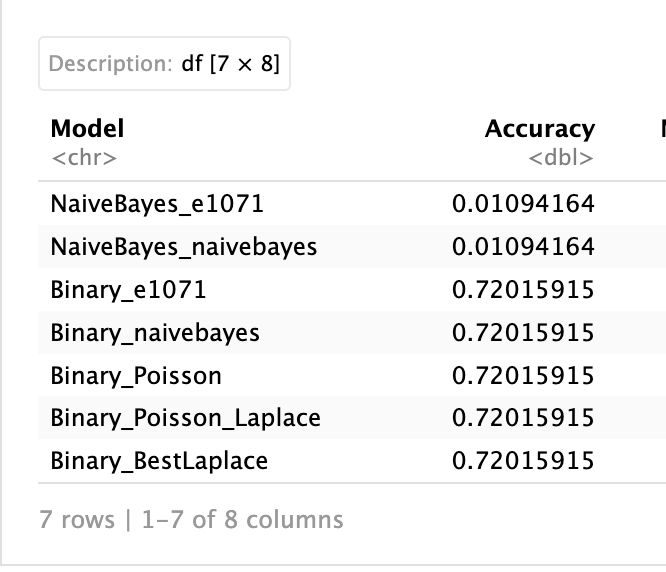
\includegraphics[width=0.9\columnwidth]{figures/summary_naive.jpeg}
    \caption{Summary of metrics}
    \label{summary}
\end{figure}

\section{Conclusions}
This study set out to investigate whether a naive Bayes classifier could  succeed in categorizing paranormal stories  obtained from the \textit{Your Ghost Stories} platform  reasonably well or not. 
Based on the models trained, the classifier implementing Laplace Smoothing achieved the highest accuracy of all with roughly 0.72. However, it is worth mentioning that this accuracy is still somewhat low and other metrics such as recall of F1 are equally low or much lower, which likely means that these classifiers are not well-suited for the dataset inspected with the word selection that was applied.

Overall, these results indicate that the naive Bayes classifier is a simple and potentially effective tool for analyzing large amounts of text in natural language in this domain. Nevertheless, there are clear limitations, including computational power for the computations involving the most frequent words (we only considered the 3000 most frequent ones) and the architecture of the method itself applied to NLP in this particular setting, which highlight the need for future refinements.

In conclusion, even though this study confirms that probabilistic models like naive Bayes could in theory provide meaningful insights into cultural data such as paranormal stories. Yet, further improvements and refinements would be crucial in order to reach higher levels of precision and an overall better performance of these models.



\section{References}

\begin{thebibliography}{9}
\setlength{\itemsep}{0pt}
\setlength{\parskip}{0pt}


\bibitem{RPubs}
RPubs - Naïve Bayes con R para clasificacion de texto. (n.d.).
\url{https://rpubs.com/jboscomendoza/naive_nayes_con_r_clasificacion_texto}

\vspace{0.3cm}


\end{thebibliography}

\end{document}
